% This file was created with tikzplotlib v0.10.1.
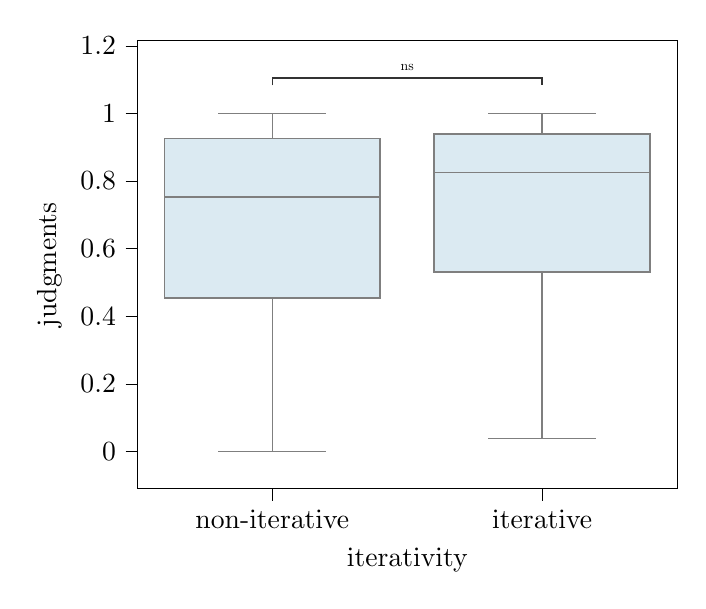
\begin{tikzpicture}

\definecolor{darkgray176}{RGB}{176,176,176}
\definecolor{darkslategray51}{RGB}{51,51,51}
\definecolor{gray127}{RGB}{127,127,127}
% \definecolor{lightgray}{RGB}{211,211,211}
\definecolor{lightgray}{RGB}{219, 234, 242}

\begin{axis}[
tick align=outside,
tick pos=left,
x grid style={darkgray176},
xlabel={iterativity},
xmin=-0.5, xmax=1.5,
xtick style={color=black},
xtick={0,1},
xticklabels={non-iterative,iterative},
y grid style={darkgray176},
ylabel={judgments},
% ymin=-0.05, ymax=1.05,
ytick style={color=black}
]
\path [draw=gray127, fill=lightgray, semithick]
(axis cs:-0.4,0.454843779675851)
--(axis cs:0.4,0.454843779675851)
--(axis cs:0.4,0.926146914181622)
--(axis cs:-0.4,0.926146914181622)
--(axis cs:-0.4,0.454843779675851)
--cycle;
\path [draw=gray127, fill=lightgray, semithick]
(axis cs:0.6,0.530266595121465)
--(axis cs:1.4,0.530266595121465)
--(axis cs:1.4,0.939695626126269)
--(axis cs:0.6,0.939695626126269)
--(axis cs:0.6,0.530266595121465)
--cycle;
\addplot [semithick, gray127]
table {%
0 0.454843779675851
0 0
};
\addplot [semithick, gray127]
table {%
0 0.926146914181622
0 1
};
\addplot [semithick, gray127]
table {%
-0.2 0
0.2 0
};
\addplot [semithick, gray127]
table {%
-0.2 1
0.2 1
};
\addplot [semithick, gray127]
table {%
1 0.530266595121465
1 0.0381659063849534
};
\addplot [semithick, gray127]
table {%
1 0.939695626126269
1 1
};
\addplot [semithick, gray127]
table {%
0.8 0.0381659063849534
1.2 0.0381659063849534
};
\addplot [semithick, gray127]
table {%
0.8 1
1.2 1
};
\addplot [semithick, darkslategray51]
table {%
0 1.083
0 1.105
1 1.105
1 1.083
};
\addplot [semithick, gray127]
table {%
-0.4 0.752545580411381
0.4 0.752545580411381
};
\addplot [semithick, gray127]
table {%
0.6 0.825657986349093
1.4 0.825657986349093
};
\draw (axis cs:0.5,1.105) ++(0pt,1pt) node[
  scale=0.5,
  anchor=south,
  text=black,
  rotate=0.0
]{ns};
\end{axis}

\end{tikzpicture}
